\documentclass[11pt]{article}
\usepackage[utf8]{inputenc}
\usepackage{tikz}
\usetikzlibrary{shapes.geometric, arrows}

\tikzstyle{startstop} =[rectangle, rounded corners, minimum width =3cm,text width=4cm, minimum height=1cm ,text centered, draw=black , fill =red!20]
\tikzstyle{io}= [trapezium, trapezium left angle =70 ,text width=3cm,trapezium right angle =110, minimum width =3cm, minimum height =1cm,text centered, draw=black, fill= blue!20]
\tikzstyle{process} =[rectangle, minimum width= 3cm , text width=4cm,minimum height =1cm , text centered, draw=black, fill = orange!50]
\tikzstyle{decision} =[diamond, minimum width =3cm,text width=1.5cm, minimum height =1cm, text centered, draw=black , fill =green!30]
\tikzstyle{arrow} =[thick,->,>=stealth]


\begin{document}

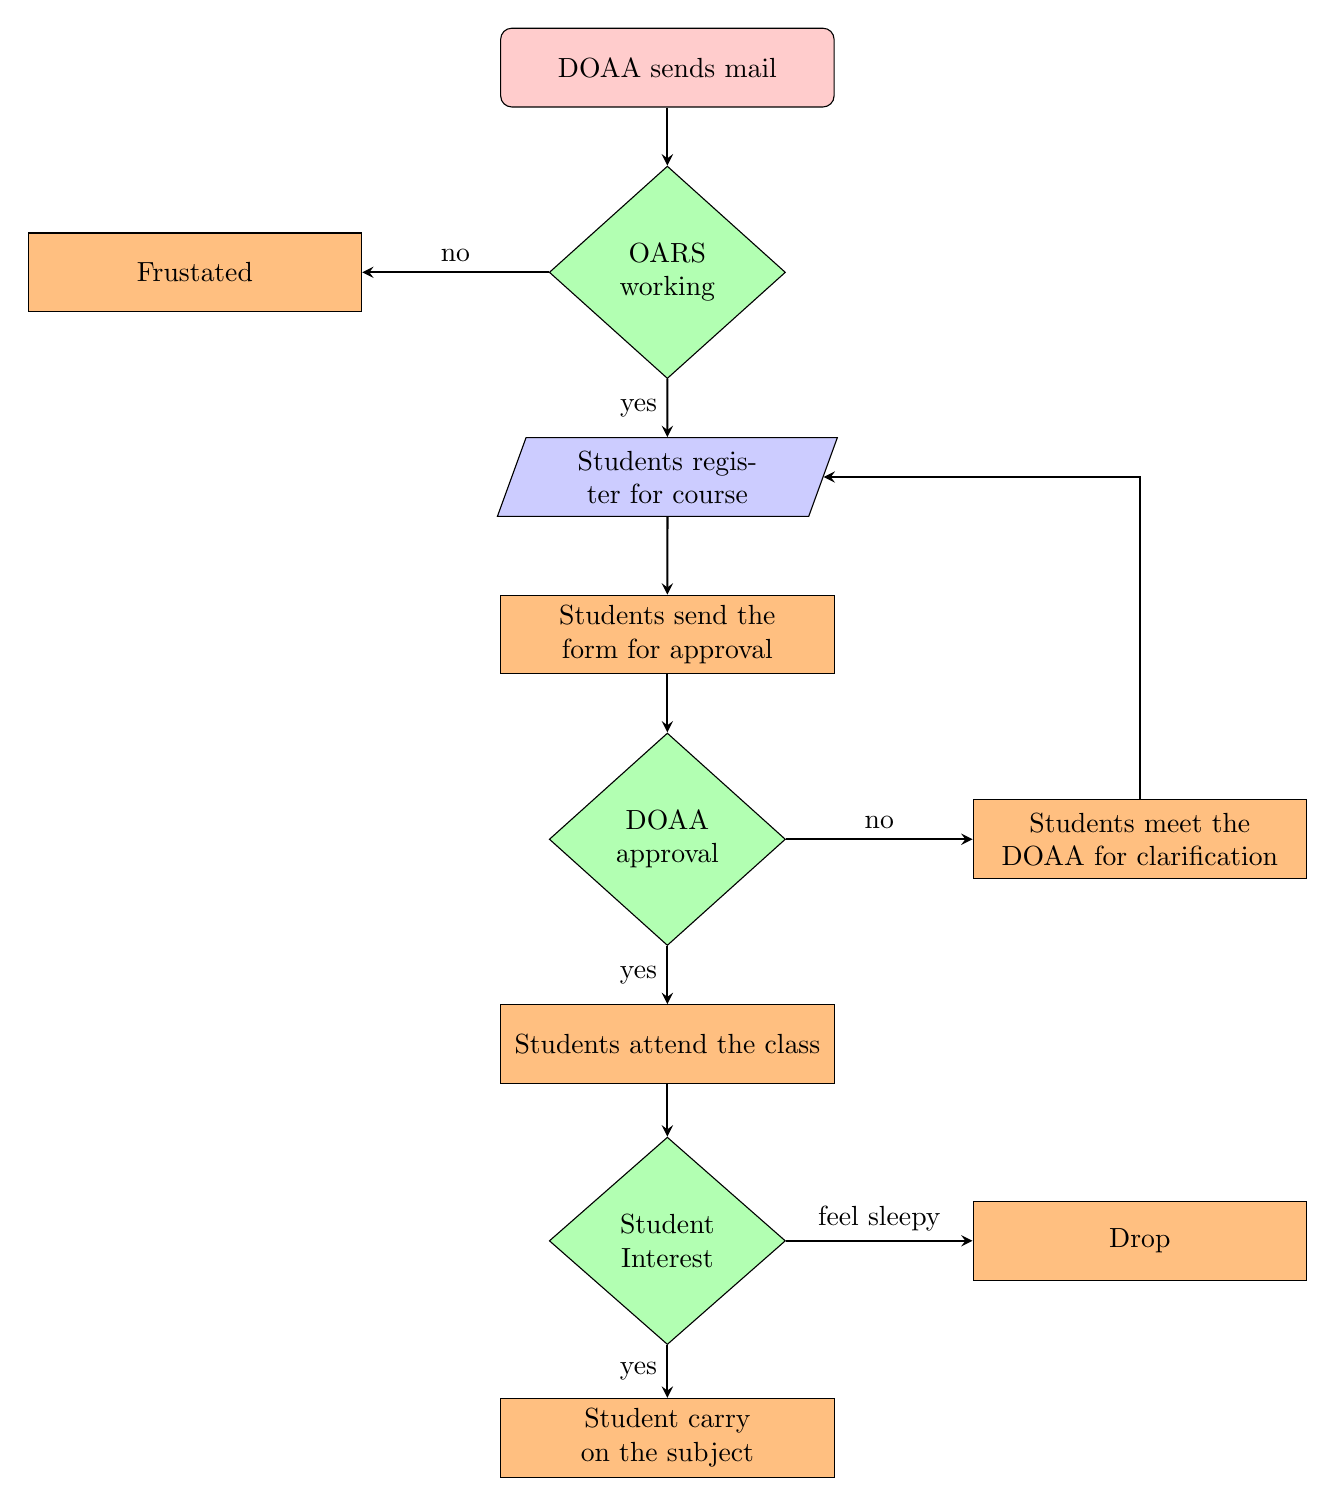
\begin{tikzpicture}[node distance=2cm]
\node (start) [startstop] {DOAA sends mail};
\node (dec2) [decision , below of=start, yshift=-0.6cm] {OARS working};
\node (in1) [io,below of=dec2, yshift= -0.6cm] {Students register for course};
\node (pro5) [process, below of=in1] {Students send the form for approval};
\node (pro1) [decision, below of=pro5, yshift= -0.6cm] {DOAA approval};
\node (pro2) [process, below of=pro1, yshift= -0.6cm] {Students attend the class};
\node (dec1) [decision , below of=pro2 , yshift=-0.5cm] {Student Interest};
\node (pro3) [process, below of= dec1, yshift= -0.5cm] {Student carry on the subject};
\node (pro4) [process, right of = dec1, xshift= 4cm] { Drop};
\node (pro6) [process, left of = dec2, xshift=-4cm] {Frustated};
\node (pro7) [process, right of = pro1, xshift=4cm] {Students meet the DOAA for clarification};
\draw [arrow] (start)--(dec2);
\draw [arrow] (dec2)--node[anchor=east]{yes}(in1);
\draw [arrow] (in1)--(pro5);
\draw [arrow] (pro5)--(pro1);
\draw [arrow] (pro1)--node[anchor=east]{yes}(pro2);
\draw [arrow] (pro2)--(dec1);
\draw [arrow] (pro1) --node[anchor=south]{no}(pro7);
\draw [arrow] (pro7)|-(in1);
\draw [arrow] (dec2)--node[anchor=south]{no}(pro6);
\draw [arrow] (dec1)--node[anchor=east]{yes}(pro3);
\draw [arrow] (dec1)--node[anchor=south]{feel sleepy}(pro4);
\end{tikzpicture}
\end{document}
